
\documentclass[11pt,twocolumn]{article}
\usepackage[a4paper,margin=0.72in]{geometry}
\usepackage[utf8]{inputenc}
\usepackage[T1]{fontenc}
\usepackage{lmodern}
\usepackage{microtype}
\usepackage{graphicx}
\usepackage{booktabs}
\usepackage{amsmath}
\usepackage{caption}
\usepackage{subcaption}
\usepackage{hyperref}
\usepackage{xcolor}
\usepackage{enumitem}
\usepackage{float}
\hypersetup{colorlinks=true,linkcolor=blue,citecolor=blue,urlcolor=blue}
\setlength{\columnsep}{0.22in}
\setlength{\parskip}{0.20em}
\setlength{\parindent}{0.9em}
\captionsetup{font=small,labelfont=bf}
\graphicspath{{../figures/}}
\title{\textbf{Ensemble Methods: Boosting vs. Bagging}\\\large From-Scratch Decision Trees, AdaBoost, Random Forests, and Unsupervised Diagnostics}
\author{İbrahim Mammadov \and Nihat Rzayev \and Fatma Mammadova \and Fidan Allahverdiyeva\\AI Academy, National AI Center -- Machine Learning Spring 2026}
\date{}
\begin{document}
\maketitle
\begin{abstract}
This project studies when boosting outperforms bagging, and when bagging is the safer choice. We implement Decision Tree, AdaBoost, Random Forest, PCA, K-Means, and DBSCAN from scratch, using scikit-learn only for permitted utilities such as metrics, train/test splitting, standardization, and reference baselines. The experimental design covers baseline tree validation, AdaBoost scaling, Random Forest scaling, head-to-head cross-validation, label-noise robustness, bias--variance decomposition, and unsupervised structure analysis. Results support the core ensemble-learning trade-off: boosting can reduce bias through sequential reweighting, while Random Forest reduces variance by averaging decorrelated high-variance trees. Random Forest is especially strong on the heterogeneous Covertype task and remains comparatively stable under noisy labels.
\end{abstract}

\section{Introduction}
Ensemble learning combines multiple weak or unstable predictors to obtain a stronger model. The two most important families are \emph{bagging} and \emph{boosting}. Bagging trains models independently on bootstrap samples and aggregates their predictions, so its primary effect is variance reduction. Boosting trains learners sequentially, reweighting or refitting toward previous errors, and therefore tends to reduce bias and training error \cite{breiman1996bagging,freund1997decision}. This project compares both principles on tabular and image-like data, focusing on the conditions under which each approach is more reliable.

The submitted repository includes source code, tests, notebooks, result tables, and figures. All major algorithms are implemented without using the corresponding scikit-learn estimators as project implementations. Reference estimators are used only for sanity checks or comparison. The final test suite confirmed 151 passing tests with one multiprocessing integration test skipped by default; coverage reporting satisfies the minimum project threshold.

\section{Methods}
\subsection{Decision Tree}
The decision tree is a CART-style classifier. At each internal node the algorithm tests binary thresholds of the form $x_j \leq t$, where $j$ is a feature index and $t$ is a midpoint between consecutive sorted feature values. Split quality is measured by impurity reduction:
\begin{equation}
\Delta I = I_P - \frac{N_L}{N} I_L - \frac{N_R}{N} I_R,
\end{equation}
where $I_P$ is parent impurity, $I_L$ and $I_R$ are child impurities, and $N_L,N_R$ are child sample counts. We support both Gini impurity, $1-\sum_c p_c^2$, and entropy, $-\sum_c p_c\log_2 p_c$. Sample-weight support is included for AdaBoost.

\subsection{AdaBoost}
AdaBoost trains weak learners sequentially. We use decision stumps as the main weak learner and implement the SAMME multiclass formulation. Training begins with uniform sample weights. For learner $m$, weighted error is
\begin{equation}
\epsilon_m = \sum_i w_i^{(m)} \mathbf{1}[h_m(x_i) \neq y_i].
\end{equation}
The learner vote is weighted by
\begin{equation}
\alpha_m = \eta\left(\log\frac{1-\epsilon_m}{\epsilon_m}+\log(K-1)\right),
\end{equation}
where $K$ is the number of classes and $\eta$ is learning rate. Misclassified samples receive larger weight in the next round. This makes AdaBoost powerful on clean structured data but can make it sensitive to mislabeled observations.

\subsection{Random Forest}
Random Forest is Person 3's main module. It combines bootstrap aggregation with node-level random feature sub-sampling \cite{breiman2001random}. For each tree, a bootstrap sample of size $N$ is drawn with replacement. Approximately $63.2\%$ of the original rows appear at least once, while about $36.8\%$ remain out-of-bag (OOB). At each node only $m=\lfloor\sqrt{p}\rfloor$ candidate features are considered by default. This feature randomization reduces correlation between trees, making averaging more effective.

The implementation includes a private CART-style tree inside \texttt{src/bagging/random\_forest.py}. This was used to keep the Random Forest module independent during parallel team development. The public classifier provides \texttt{fit}, \texttt{predict}, \texttt{predict\_proba}, OOB scoring, impurity-based feature importances, deterministic per-tree seeds, and process-based tree-level parallelism through \texttt{multiprocessing.Pool}. The public \texttt{predict} method uses hard majority vote, while \texttt{predict\_proba} averages class-probability vectors. A rare-class edge case is handled explicitly: if a bootstrap tree never observes a minority class, its local probability columns are aligned to the forest-wide class list before averaging.

\subsection{Unsupervised Diagnostics}
The unsupervised part implements PCA, K-Means, and DBSCAN without using scikit-learn implementations. PCA is computed via covariance eigendecomposition, K-Means via Lloyd's algorithm with multiple restarts, and DBSCAN via density-reachable expansion of core points \cite{pearson1901pca,macqueen1967kmeans,ester1996dbscan}. These methods do not directly compete with the supervised ensembles, but they help explain the structure and separability of the datasets.

\section{Data and Reproducibility}
The repository uses local data files prepared by the download scripts. The Random Forest utilities read WDBC from \texttt{data/wdbc.data}, MNIST 3-vs-8 from \texttt{data/mnist\_3\_vs\_8.npz}, and a Covertype type-4 one-vs-rest task from \texttt{data/covtype.data}. The raw datasets should not be committed; they are reproducible through the provided scripts. All train/test splits are seeded with \texttt{random\_state}. Standardization is fitted only on the training split to avoid leakage. Severe imbalance treatment, when used, is applied only to the training data so the test distribution remains realistic.

\section{Experimental Design}
The project contains seven required experiments. Baseline validation compares the custom tree and stump with a scikit-learn reference. AdaBoost scaling evaluates staged performance as the number of estimators increases. Random Forest scaling evaluates both \texttt{n\_estimators} and \texttt{max\_depth}, tracking test accuracy, macro F1, ROC-AUC, minority recall, OOB accuracy, and runtime. Head-to-head evaluation uses five-fold cross-validation under fixed estimator budgets. Noise robustness flips training labels at 5\%, 10\%, and 20\%, keeping the test labels clean. Bias--variance decomposition estimates the role of model complexity. Finally, unsupervised analysis uses PCA, elbow curves, k-distance plots, ARI, and noise fraction.

\section{Results}
\subsection{Baseline and AdaBoost Scaling}
Table~\ref{tab:baseline} verifies that the custom decision tree is close to the scikit-learn tree reference on WDBC. The stump is intentionally weaker, which is desirable for AdaBoost.
\begin{table}[H]
\centering
\caption{Baseline tree validation on WDBC.}
\label{tab:baseline}
\resizebox{\columnwidth}{!}{
\begin{tabular}{llll}
\toprule
Model & Acc. & Macro F1 & AUC \\ 
\midrule
MyTree & 0.930 & 0.924 & 0.920 \\ 
MyStump & 0.877 & 0.860 & 0.843 \\ 
sklearn & 0.930 & 0.925 & 0.925 \\ 
\bottomrule
\end{tabular}
}
\end{table}

Table~\ref{tab:ada} summarizes the best AdaBoost staged result on each dataset. AdaBoost reaches very high accuracy on WDBC and useful performance on Adult, but Covertype remains difficult because of multiclass structure and imbalance.
\begin{table}[H]
\centering
\caption{Best AdaBoost scaling result by dataset.}
\label{tab:ada}
\resizebox{\columnwidth}{!}{
\begin{tabular}{llll}
\toprule
Dataset & Best T & Acc. & Macro F1 \\ 
\midrule
Adult & 160 & 0.853 & 0.778 \\ 
Covertype & 55 & 0.528 & 0.341 \\ 
WDBC & 30 & 0.982 & 0.981 \\ 
\bottomrule
\end{tabular}
}
\end{table}

\begin{figure}[H]
\centering
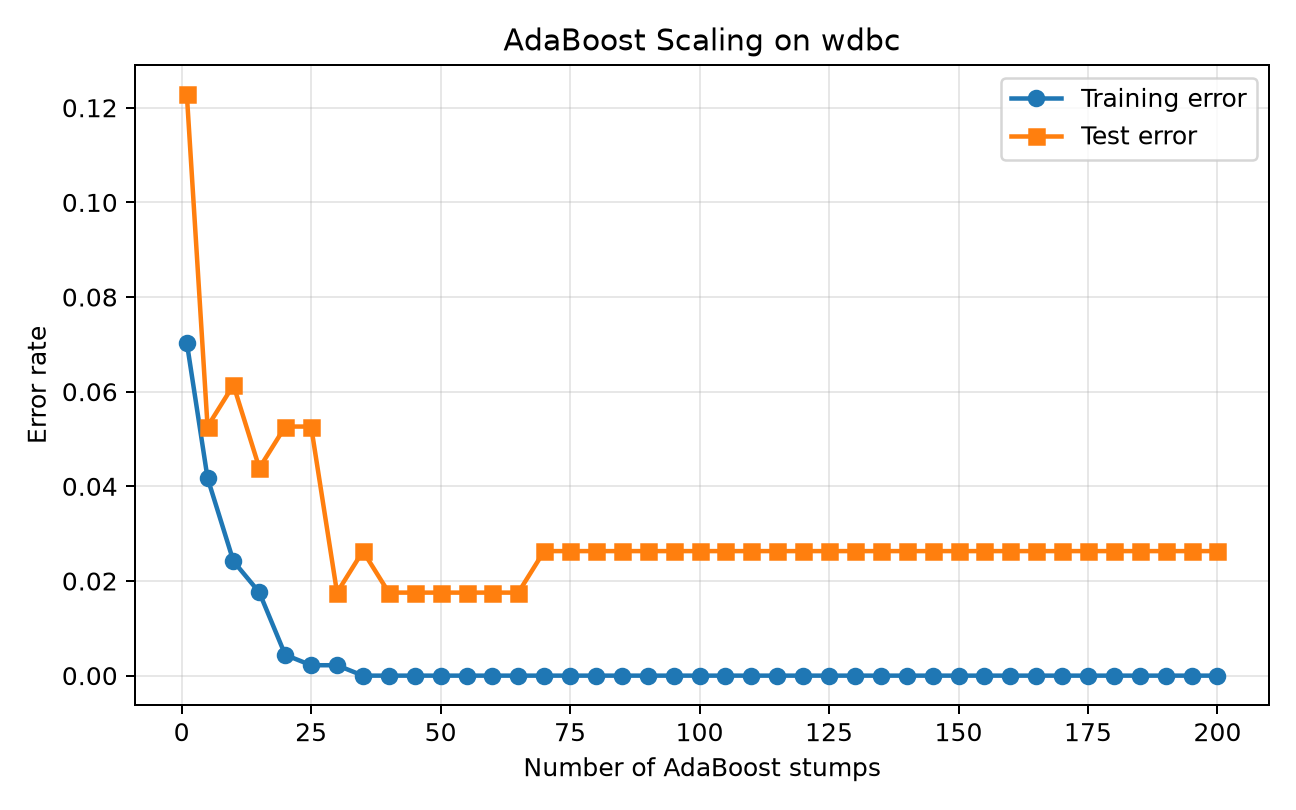
\includegraphics[width=\columnwidth]{adaboost_scaling_wdbc.png}
\caption{AdaBoost scaling on WDBC. Staged training performance improves rapidly and test performance stabilizes once sufficient stumps are added.}
\label{fig:ada}
\end{figure}

\subsection{Random Forest Scaling}
Random Forest results show the expected bagging behavior. Increasing tree count stabilizes predictions and OOB estimates; increasing depth initially reduces underfitting but eventually gives diminishing returns. Table~\ref{tab:rfbest} summarizes the strongest point in each RF sweep.
\begin{table}[H]
\centering
\caption{Best Random Forest scaling points by dataset and sweep.}
\label{tab:rfbest}
\resizebox{\columnwidth}{!}{
\begin{tabular}{llllll}
\toprule
Dataset & Sweep & Param & Acc. & F1 & OOB \\ 
\midrule
WDBC & max depth & depth=4 & 0.958 & 0.955 & 0.955 \\ 
WDBC & n estimators & trees=50 & 0.958 & 0.955 & 0.953 \\ 
Covertype type-4 & max depth & depth=14 & 0.996 & 0.819 & 0.998 \\ 
Covertype type-4 & n estimators & trees=10 & 0.997 & 0.833 & 0.998 \\ 
Digits 3-vs-8 & max depth & depth=7 & 0.989 & 0.989 & 0.985 \\ 
Digits 3-vs-8 & n estimators & trees=40 & 0.989 & 0.989 & 0.981 \\ 
\bottomrule
\end{tabular}
}
\end{table}

\begin{figure*}[t]
\centering
\begin{subfigure}{0.48\textwidth}
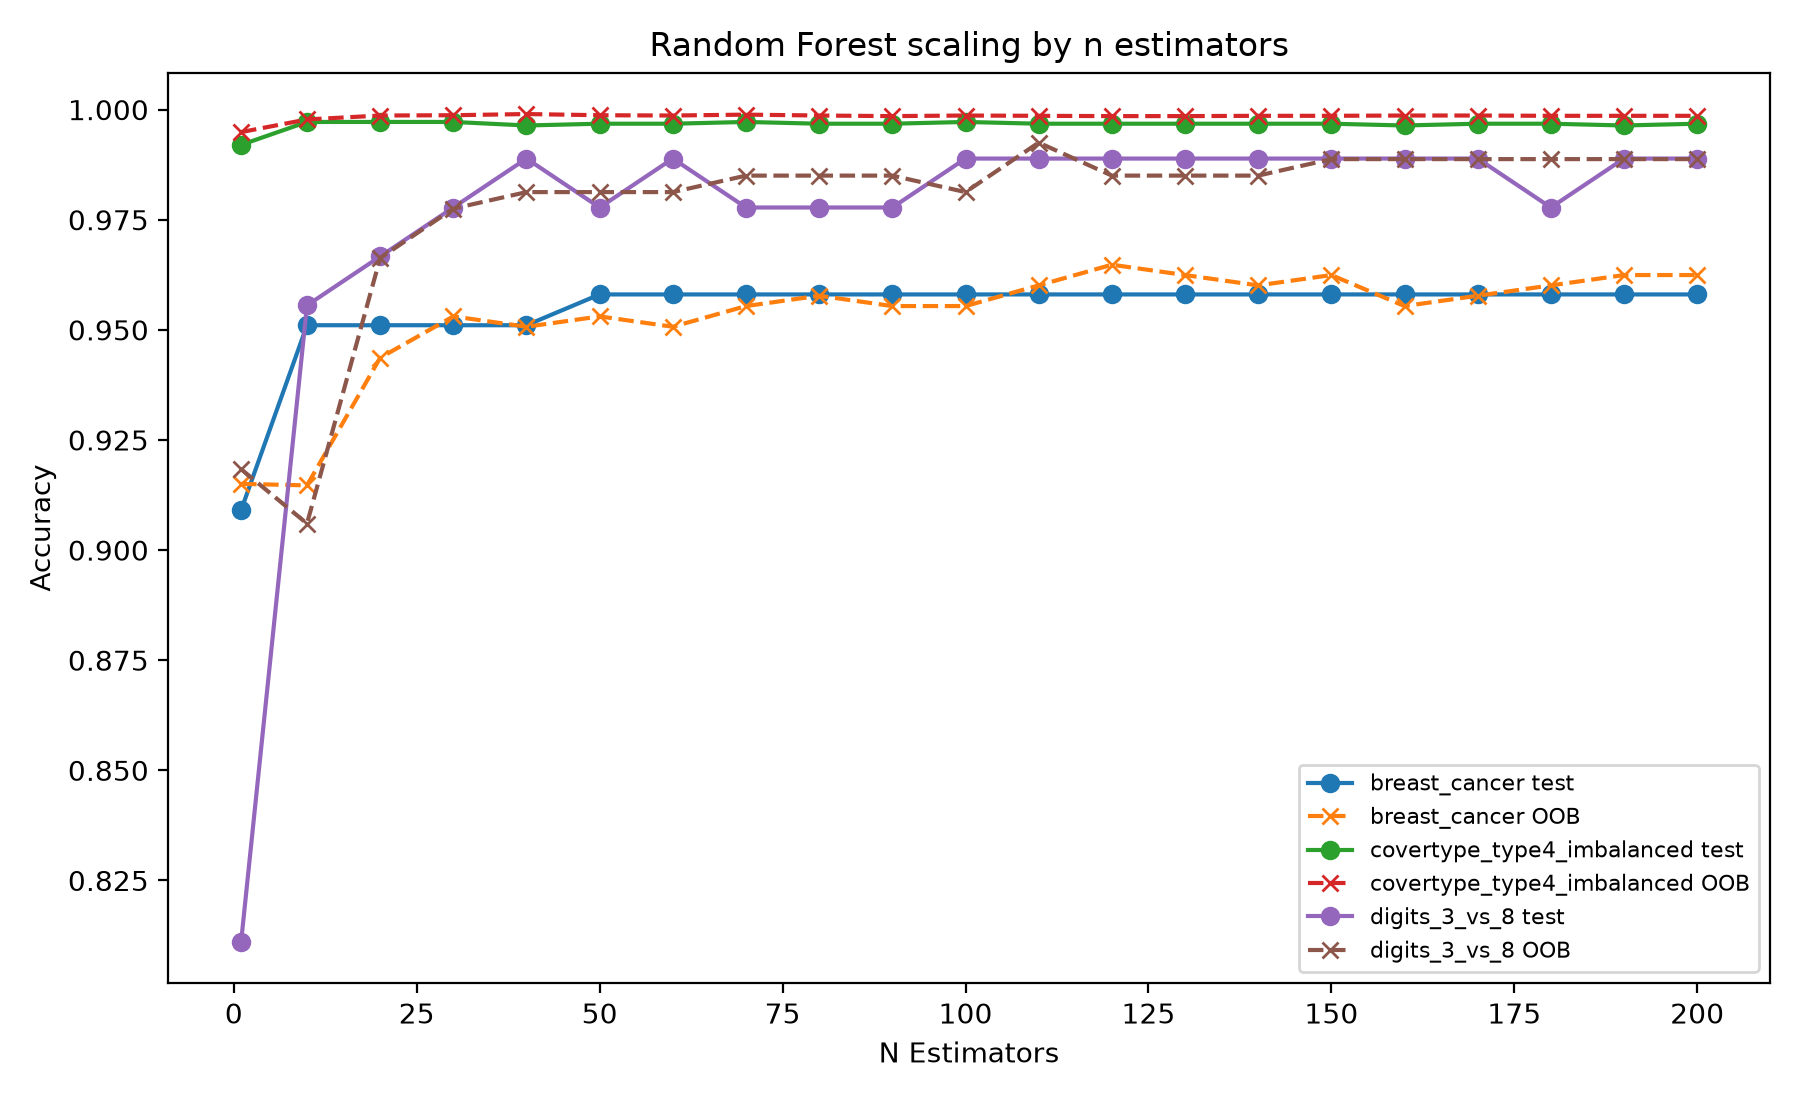
\includegraphics[width=\linewidth]{rf_scaling_n_estimators.png}
\caption{Estimator-count sweep.}
\end{subfigure}\hfill
\begin{subfigure}{0.48\textwidth}
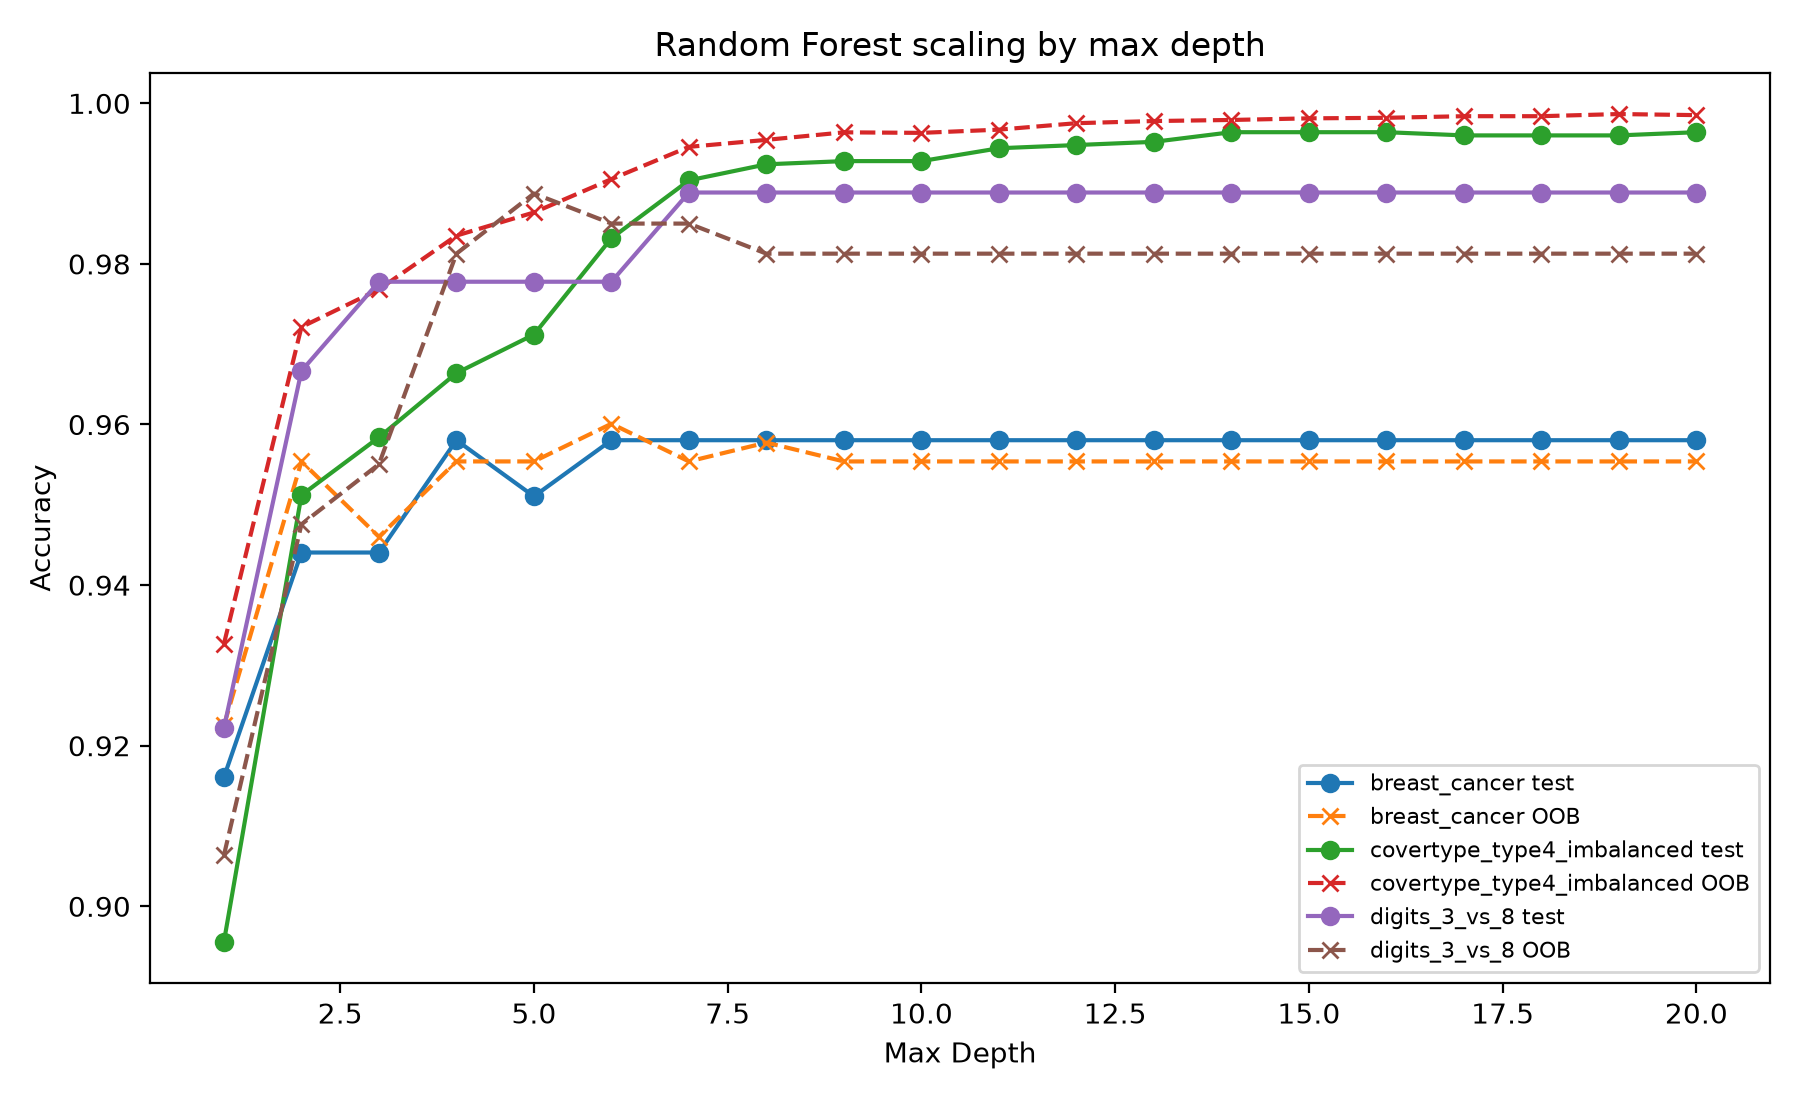
\includegraphics[width=\linewidth]{rf_scaling_max_depth.png}
\caption{Depth sweep.}
\end{subfigure}
\caption{Random Forest scaling. The test/OOB curves become stable once enough independent bootstrap trees are averaged.}
\label{fig:rfscale}
\end{figure*}

\subsection{Head-to-Head Comparison}
Table~\ref{tab:h2h} compares AdaBoost, bonus SAMME.R, and Random Forest with five-fold cross-validation. WDBC is strong for all models, Adult is close, and Covertype strongly favors Random Forest. This supports the interpretation that bagging is valuable when tabular structure is heterogeneous and tree variance needs stabilization.
\begin{table*}[t]
\centering
\caption{Five-fold head-to-head results. Values are cross-validation means.}
\label{tab:h2h}
\begin{tabular}{lllll}
\toprule
Dataset & Model & Accuracy & Macro F1 & ROC-AUC \\
\midrule
WDBC & AdaBoost & 0.967 & 0.964 & 0.993 \\ 
WDBC & AdaBoost SAMME.R bonus & 0.970 & 0.968 & 0.995 \\ 
WDBC & Random Forest & 0.956 & 0.953 & 0.988 \\ 
Adult & AdaBoost & 0.848 & 0.774 & 0.906 \\ 
Adult & AdaBoost SAMME.R bonus & 0.856 & 0.790 & 0.913 \\ 
Adult & Random Forest & 0.849 & 0.780 & 0.902 \\ 
Covertype & AdaBoost & 0.483 & 0.359 & 0.864 \\ 
Covertype & AdaBoost SAMME.R bonus & 0.446 & 0.389 & 0.870 \\ 
Covertype & Random Forest & 0.829 & 0.797 & 0.982 \\
\bottomrule
\end{tabular}
\end{table*}

\begin{figure}[H]
\centering
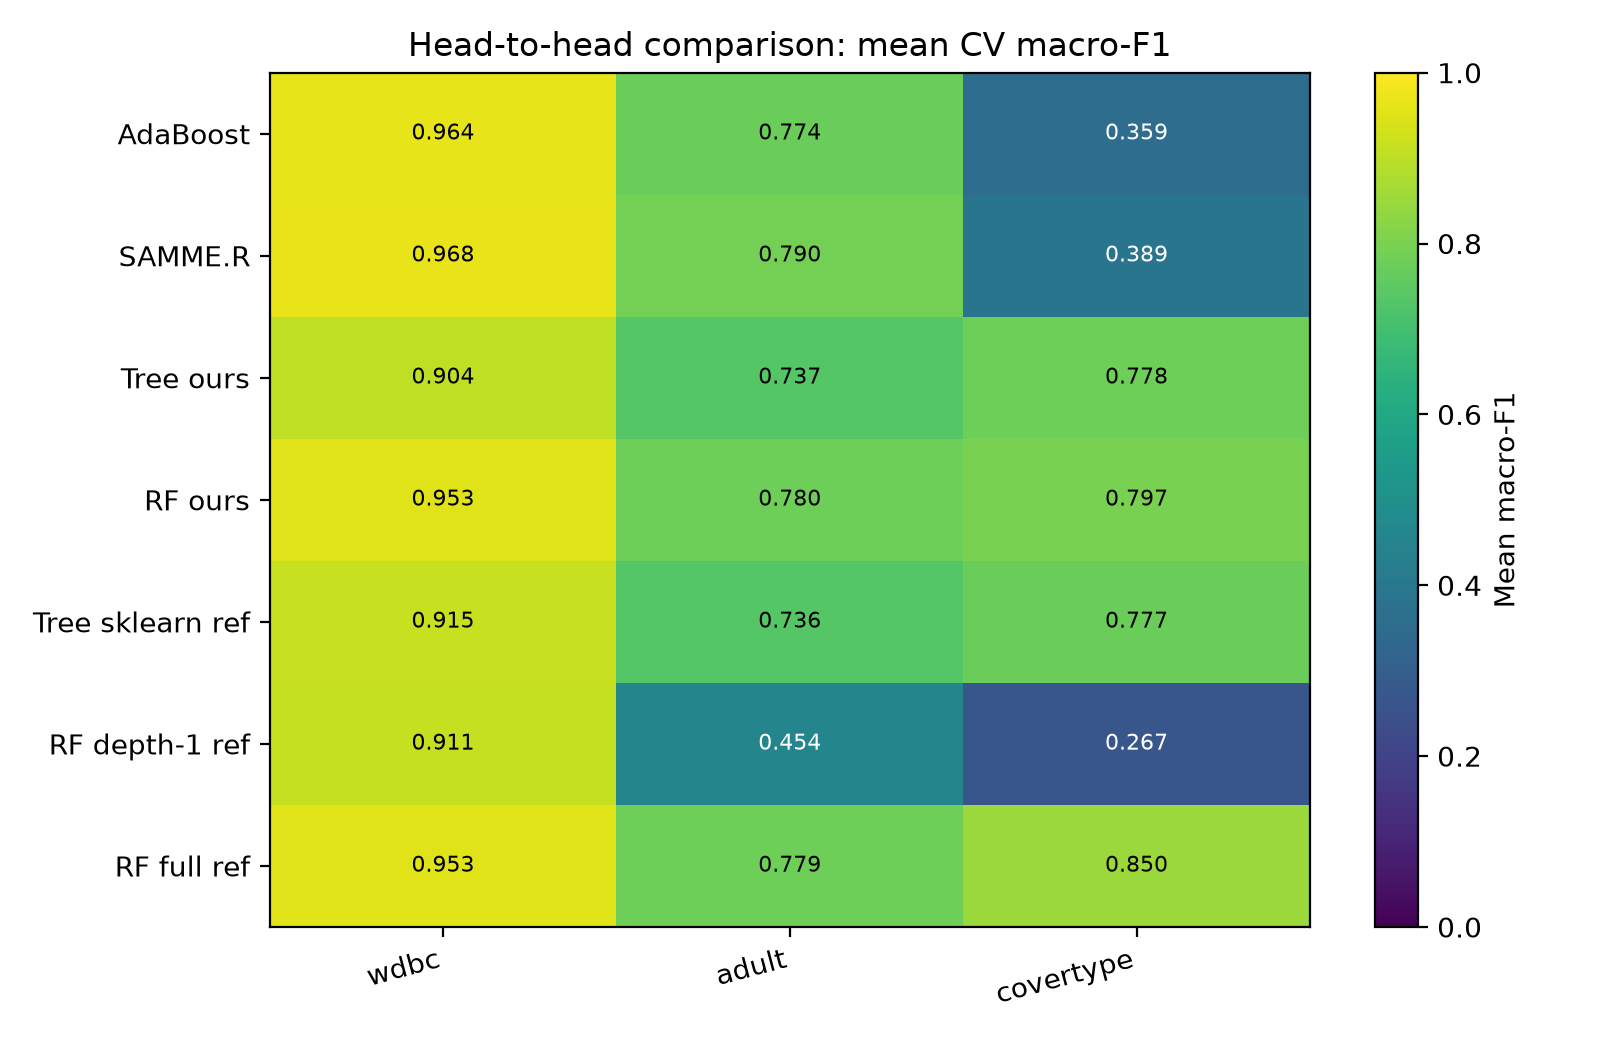
\includegraphics[width=\columnwidth]{head_to_head_macro_f1.png}
\caption{Head-to-head macro F1. Random Forest is clearly strongest on Covertype, while WDBC and Adult are closer.}
\label{fig:h2h}
\end{figure}

\subsection{Noise Robustness}
The noise experiment corrupts only training labels and evaluates on clean test labels. Table~\ref{tab:noise} shows accuracy drops at 20\% noise. AdaBoost often loses more because sequential reweighting can emphasize mislabeled examples. Random Forest spreads noise across bootstrap samples and averages it out, though it is not immune.
\begin{table}[H]
\centering
\caption{Clean-test accuracy under 20\% noisy training labels.}
\label{tab:noise}
\resizebox{\columnwidth}{!}{
\begin{tabular}{lllll}
\toprule
Dataset & Model & 0\% & 20\% & Drop \\ 
\midrule
WDBC & adaboost & 0.965 & 0.874 & 0.091 \\ 
WDBC & random forest & 0.958 & 0.944 & 0.014 \\ 
Covertype type-4 & adaboost & 0.991 & 0.647 & 0.344 \\ 
Covertype type-4 & random forest & 0.992 & 0.707 & 0.285 \\ 
Digits 3-vs-8 & adaboost & 0.967 & 0.789 & 0.178 \\ 
Digits 3-vs-8 & random forest & 0.989 & 0.922 & 0.067 \\ 
\bottomrule
\end{tabular}
}
\end{table}

\begin{figure}[H]
\centering
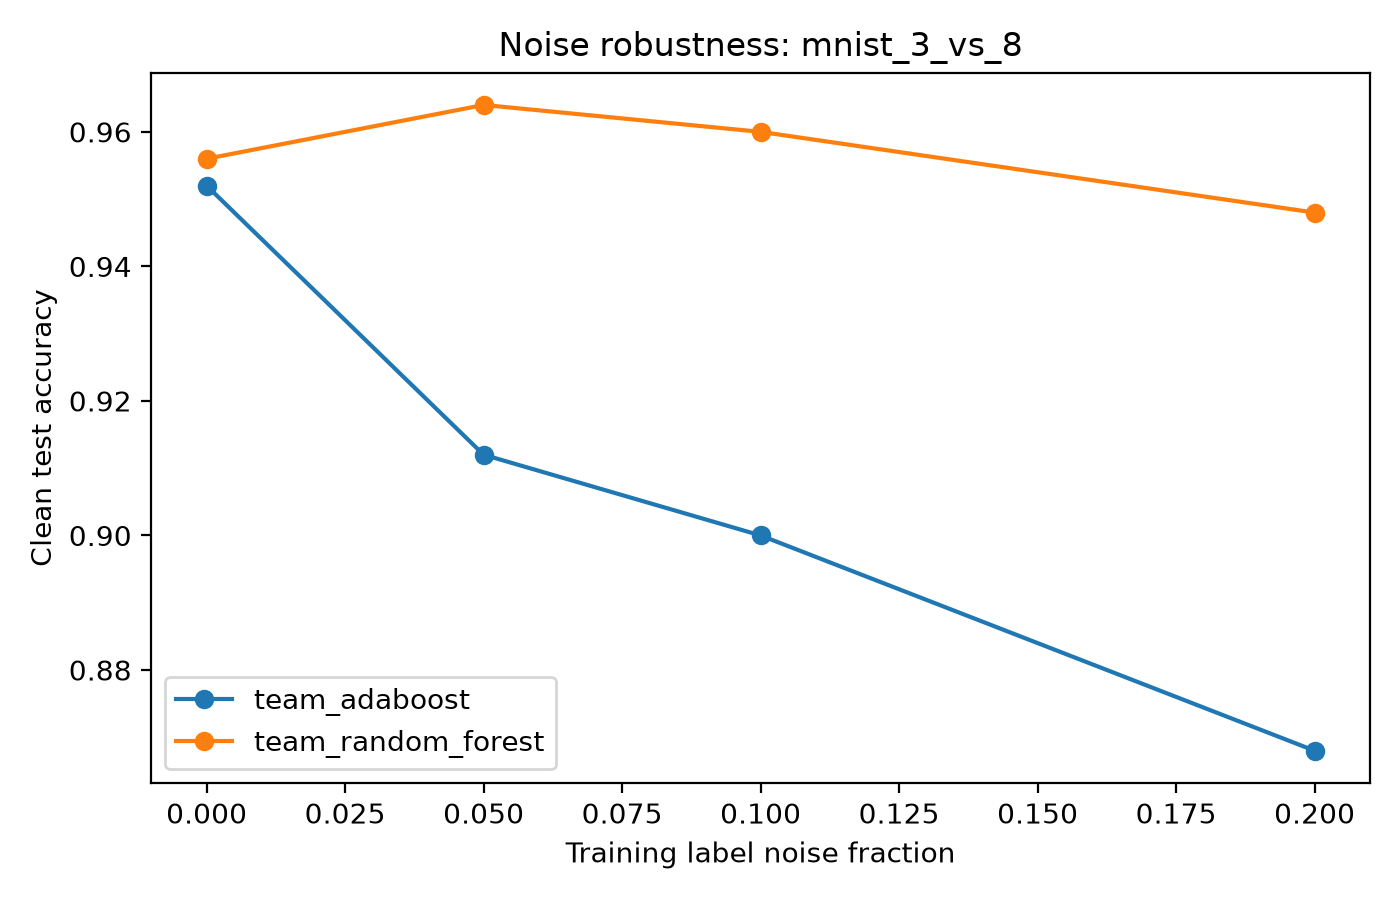
\includegraphics[width=\columnwidth]{noise_robustness_mnist_3_vs_8.png}
\caption{Noise robustness on high-dimensional MNIST 3-vs-8. Random Forest remains more stable than AdaBoost at higher label-noise levels.}
\label{fig:noise}
\end{figure}

\subsection{Bias--Variance and Unsupervised Results}
The bias--variance experiment supports the high-level story: a stump has high bias, AdaBoost reduces bias, and Random Forest stabilizes high-variance trees. The unsupervised results show that a two-dimensional PCA projection explains only part of MNIST structure, and K-Means produces better clustering structure than DBSCAN under the selected parameters.
\begin{table}[H]
\centering
\caption{Bias--variance decomposition on WDBC.}
\label{tab:bv}
\resizebox{\columnwidth}{!}{
\begin{tabular}{llll}
\toprule
Model & Loss & Bias\textasciicircum{}2 & Var. \\ 
\midrule
Decision stump & 0.084 & 0.074 & 0.053 \\ 
AdaBoost & 0.033 & 0.025 & 0.020 \\ 
Random Forest ref & 0.041 & 0.032 & 0.022 \\ 
Random Forest & 0.041 & 0.035 & 0.022 \\ 
\bottomrule
\end{tabular}
}
\end{table}

\begin{figure}[H]
\centering
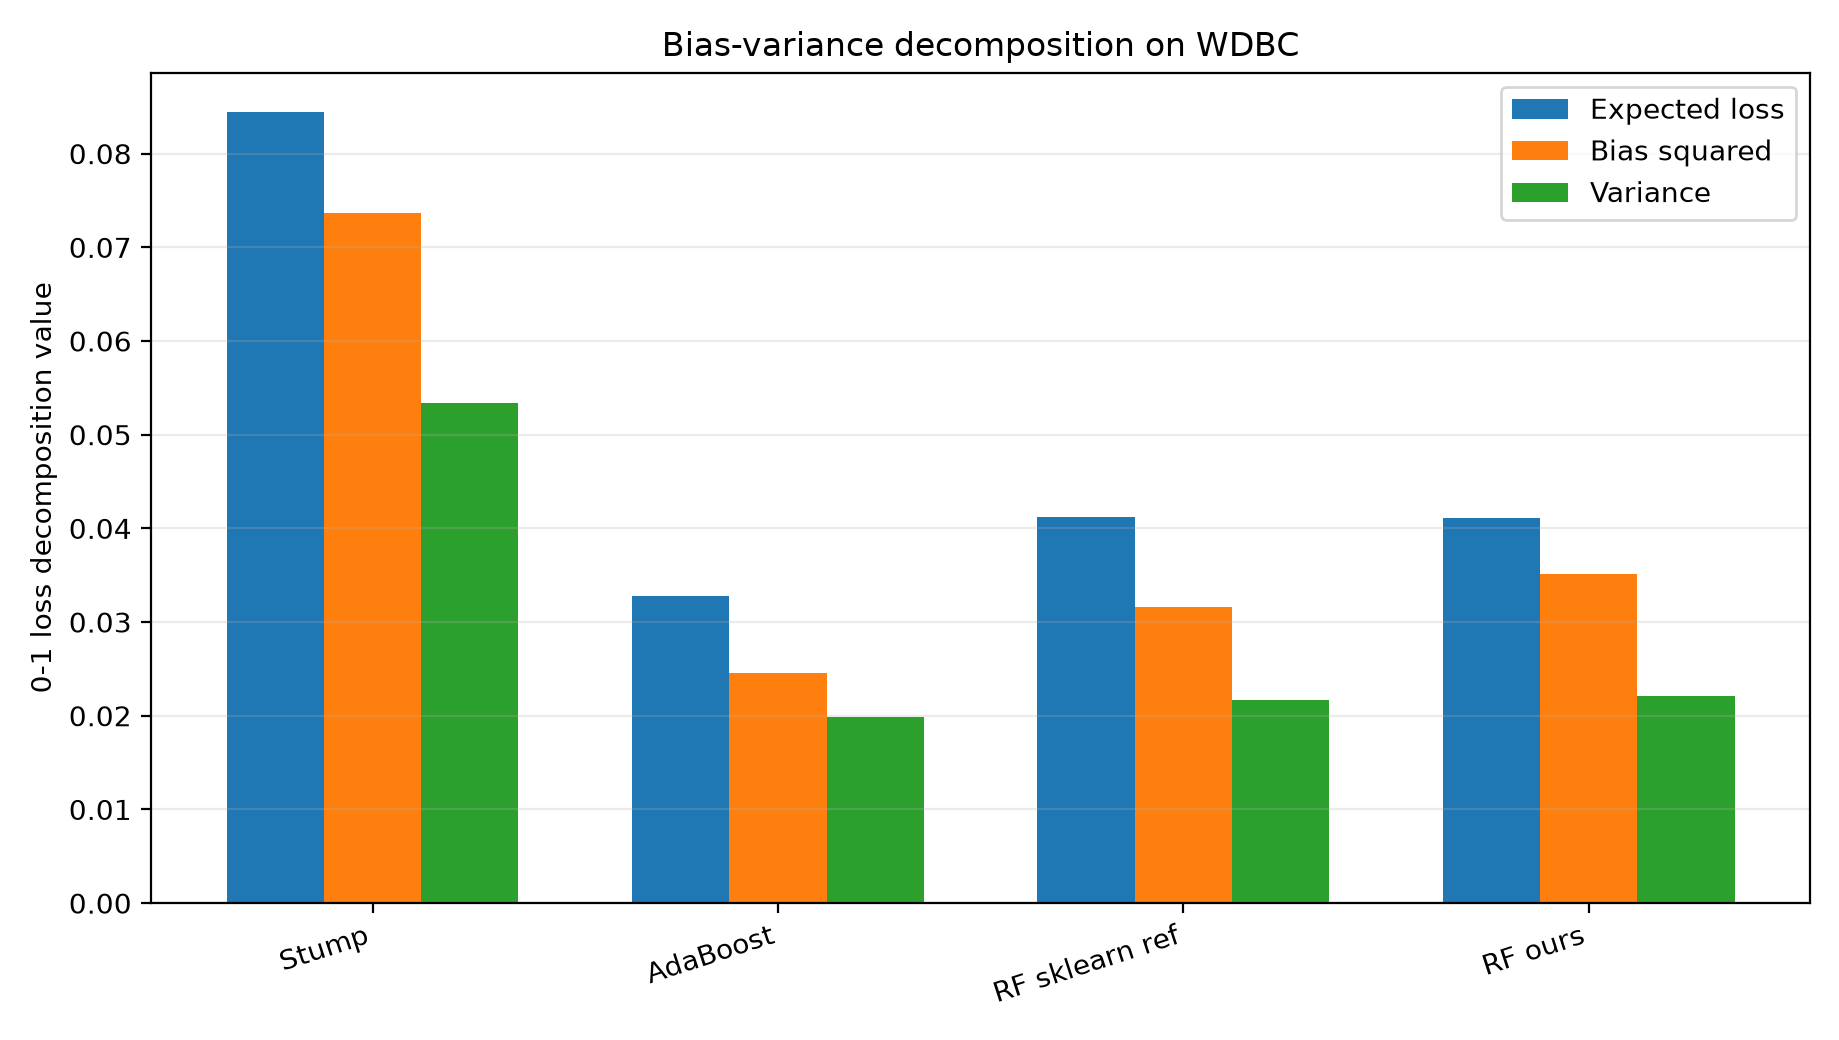
\includegraphics[width=\columnwidth]{bias_variance_decomposition.png}
\caption{Bias--variance decomposition. Boosting lowers bias, while Random Forest reduces the instability of high-variance tree learners.}
\label{fig:bv}
\end{figure}

\begin{figure*}[t]
\centering
\begin{subfigure}{0.48\textwidth}
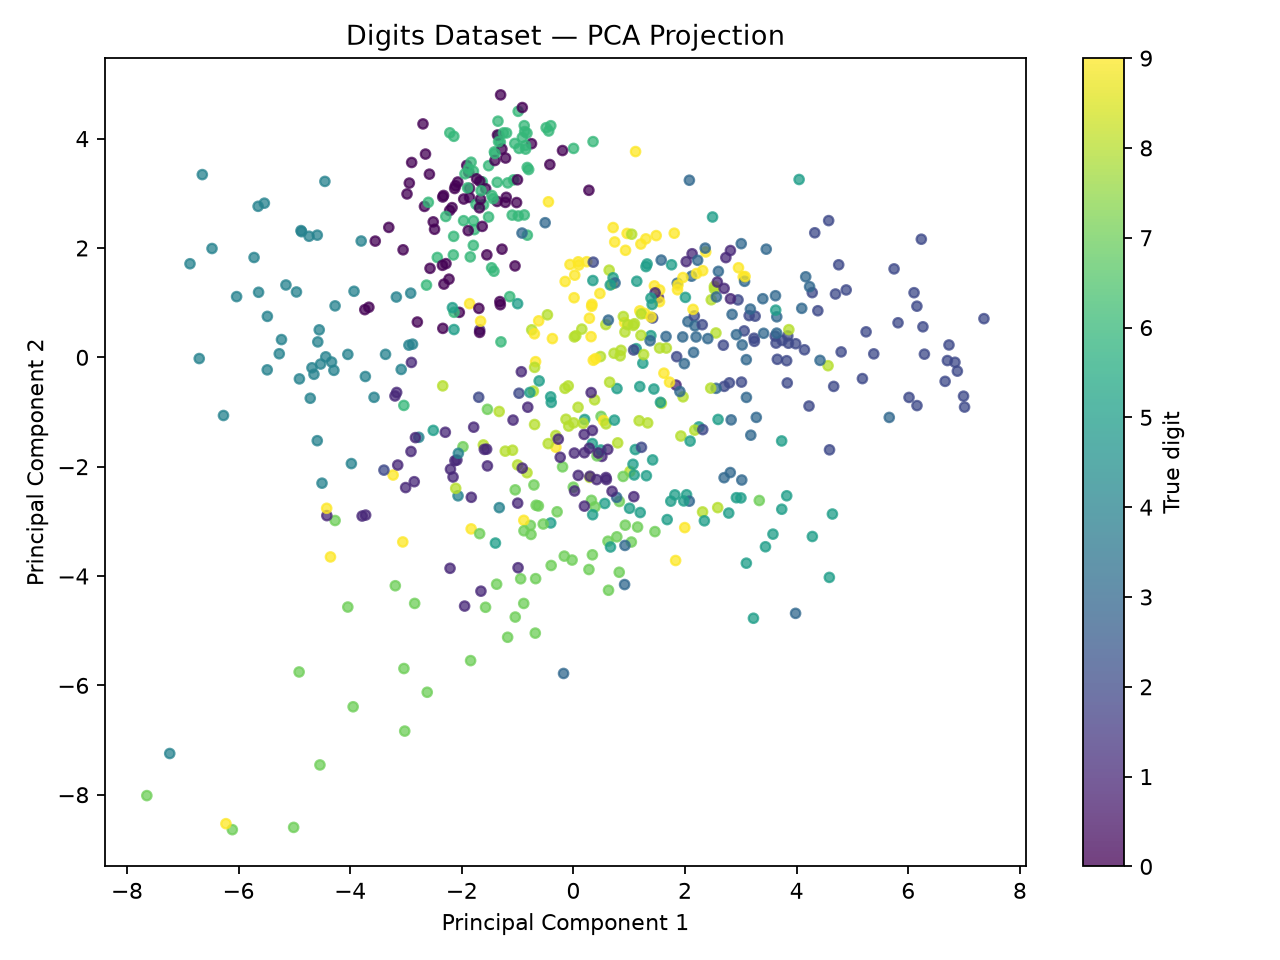
\includegraphics[width=\linewidth]{unsupervised_pca_projection.png}
\caption{PCA projection.}
\end{subfigure}\hfill
\begin{subfigure}{0.48\textwidth}
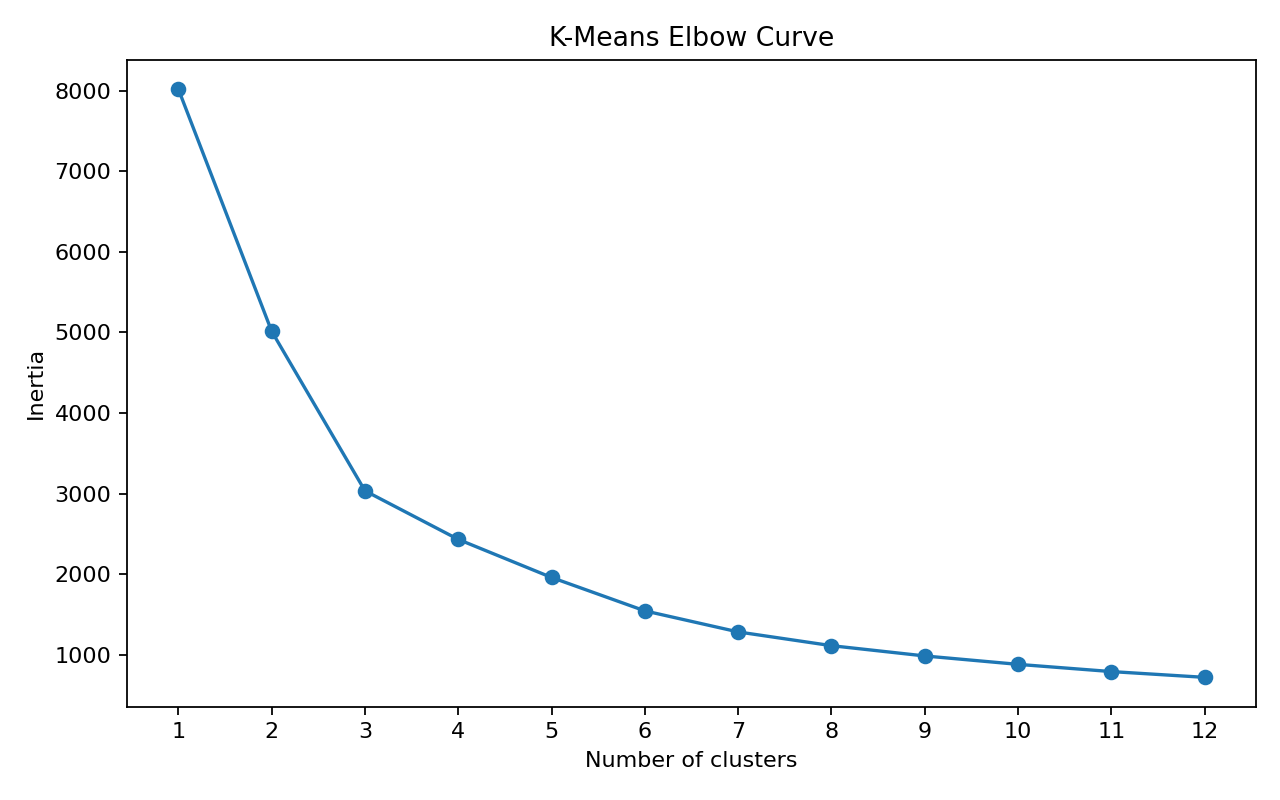
\includegraphics[width=\linewidth]{unsupervised_kmeans_elbow.png}
\caption{K-Means elbow.}
\end{subfigure}
\caption{Unsupervised diagnostics. Two PCA dimensions preserve limited variance, and the elbow curve supports the need for nonlinear supervised models.}
\end{figure*}


\subsection{Additional Noise and Bonus Diagnostics}
The same noise protocol was also applied to WDBC and Covertype. The WDBC result is useful because the dataset is small and clean; the Covertype result is useful because the minority class is rare and accuracy can be misleading. These two settings show why the report tracks macro F1, minority recall, and ROC-AUC in addition to accuracy.

\begin{figure*}[t]
\centering
\begin{subfigure}{0.32\textwidth}
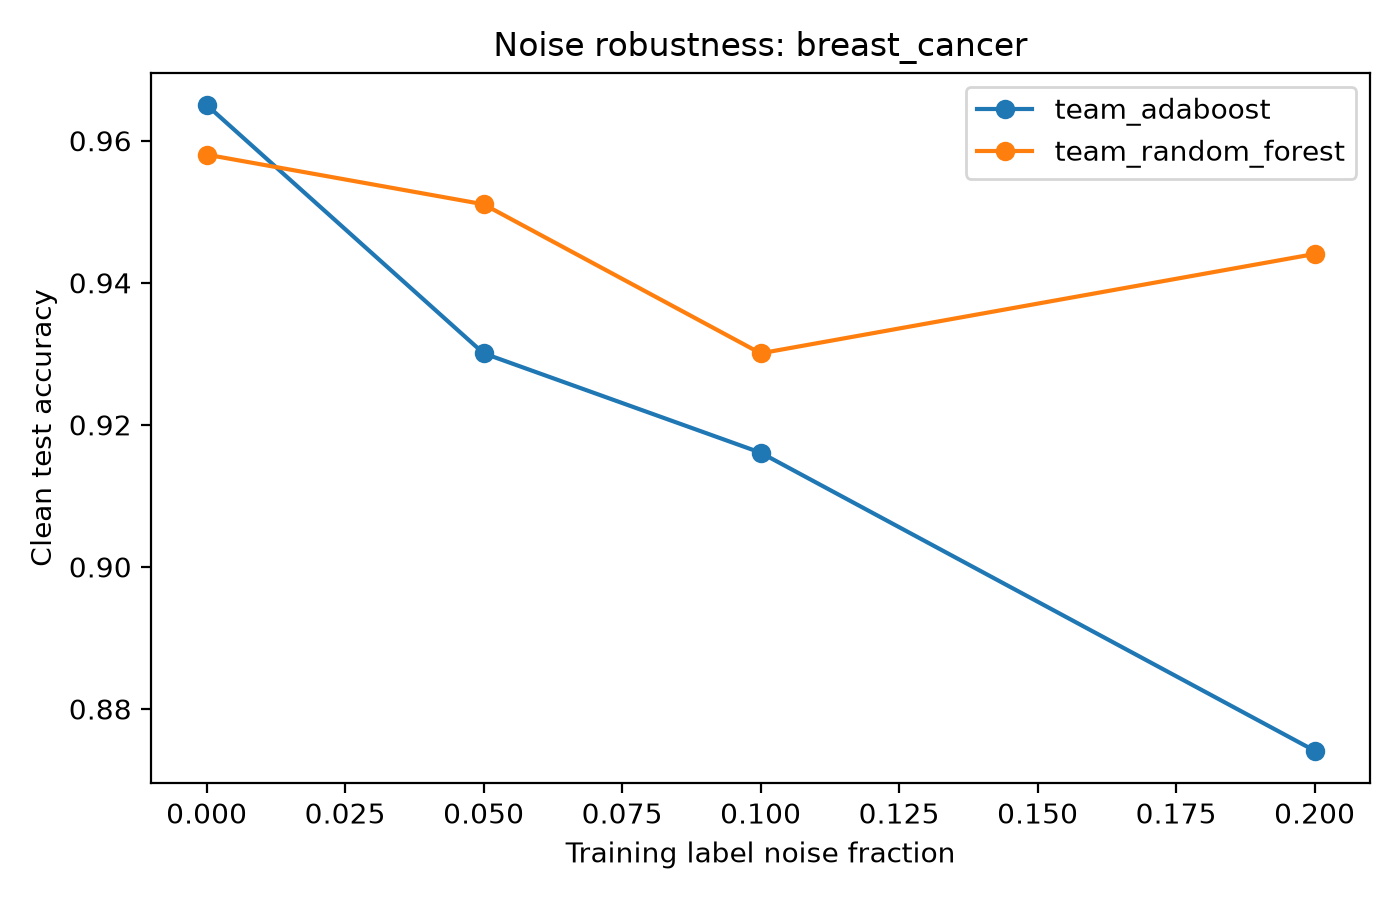
\includegraphics[width=\linewidth]{noise_robustness_breast_cancer.png}
\caption{WDBC.}
\end{subfigure}\hfill
\begin{subfigure}{0.32\textwidth}
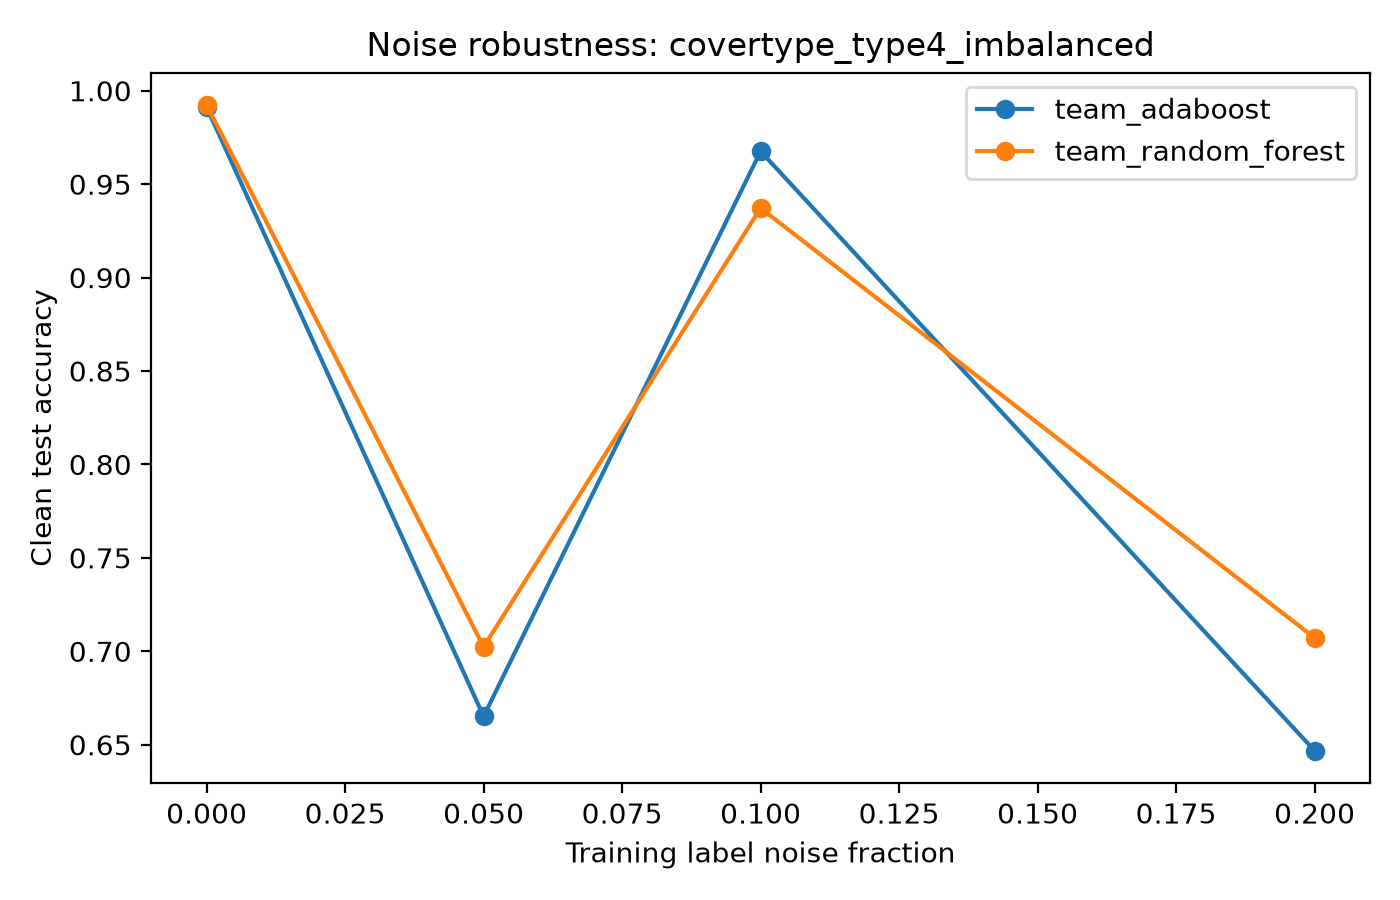
\includegraphics[width=\linewidth]{noise_robustness_covertype_type4_imbalanced.png}
\caption{Covertype type-4.}
\end{subfigure}\hfill
\begin{subfigure}{0.32\textwidth}
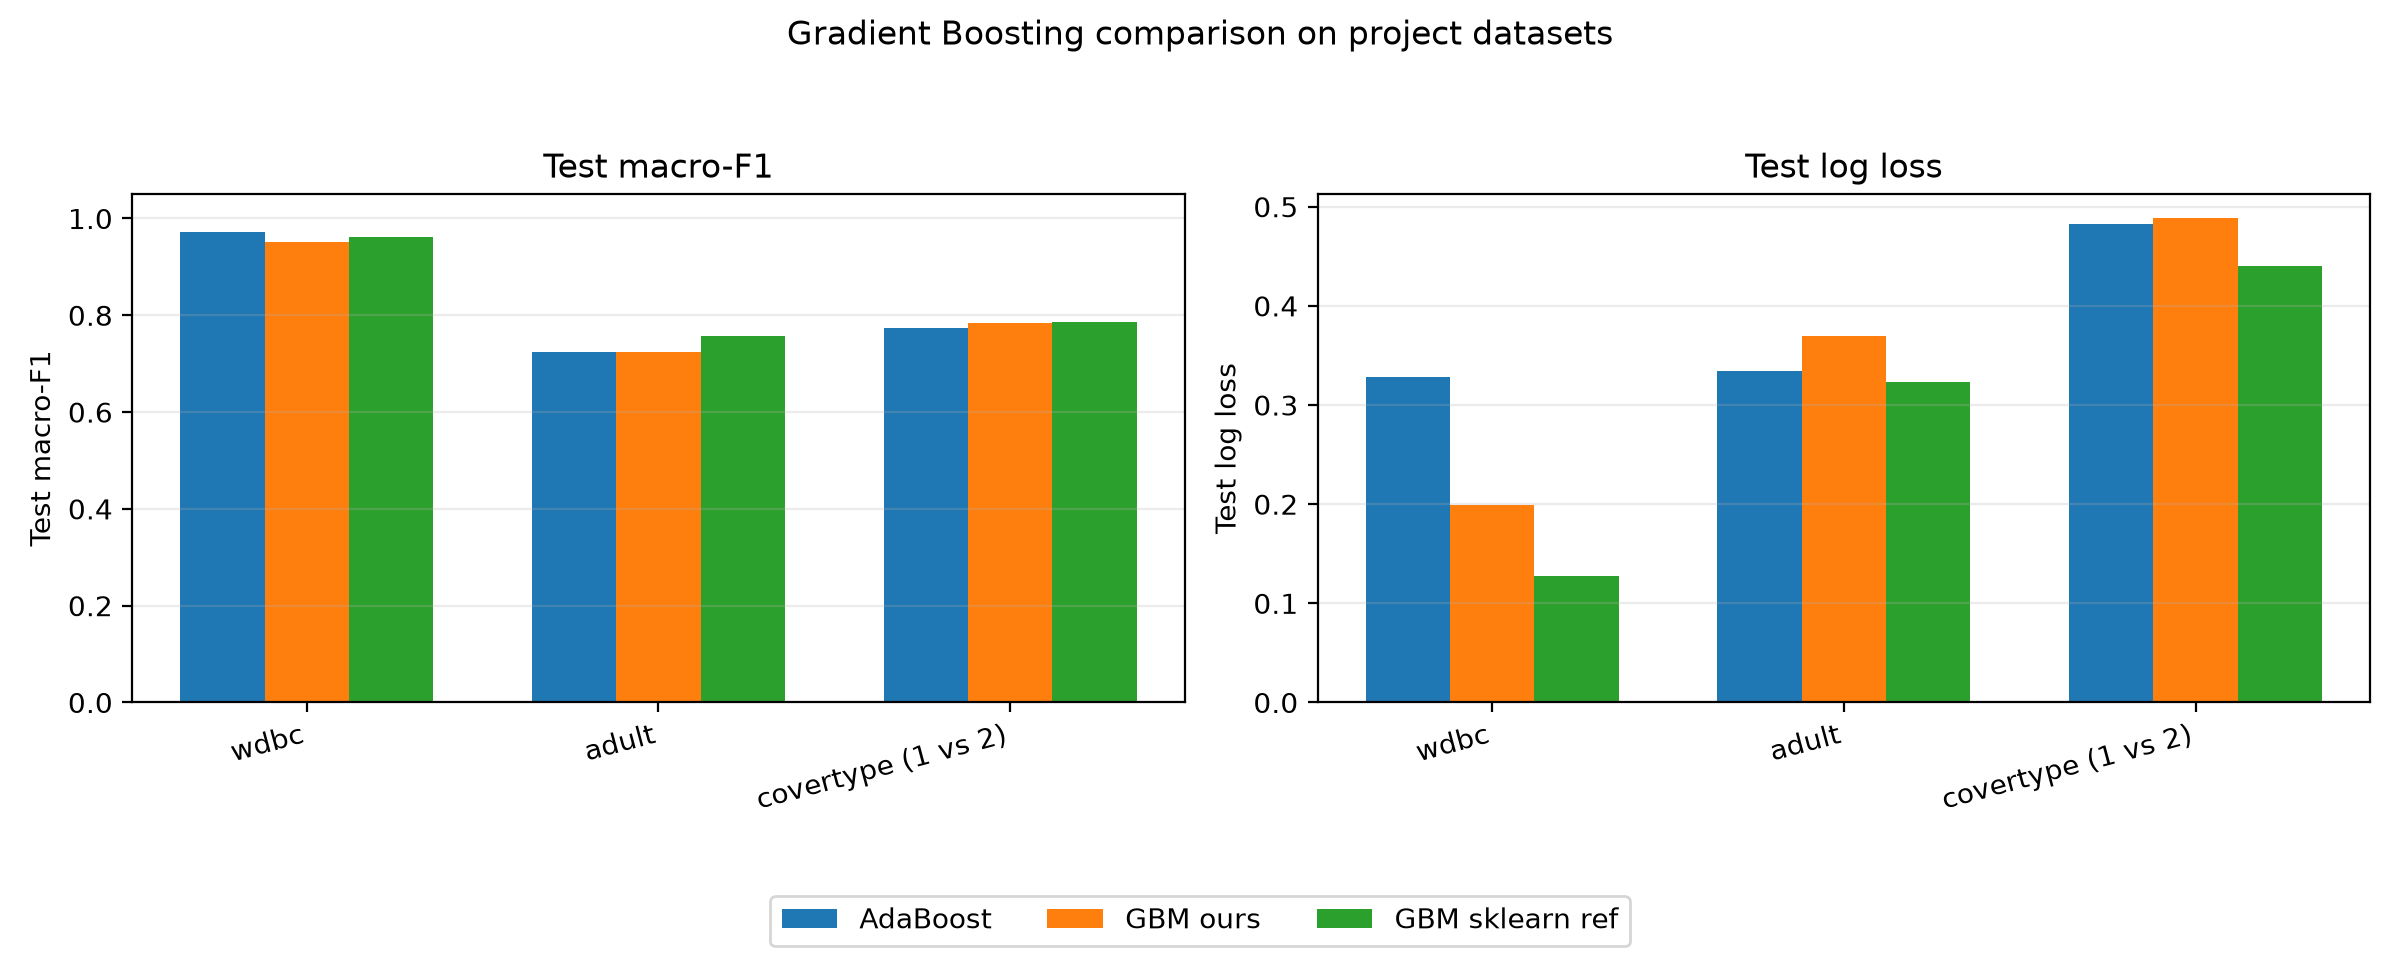
\includegraphics[width=\linewidth]{gbm_comparison_metrics.png}
\caption{GBM bonus comparison.}
\end{subfigure}
\caption{Additional robustness and bonus diagnostics. The high-dimensional and imbalanced settings demonstrate why a single accuracy number is not enough.}
\end{figure*}

\section{Implementation Details}
\subsection{Random Forest Code Path}
The Random Forest module is organized into a private tree layer and a public ensemble layer. The private \texttt{\_CARTClassificationTree} performs recursive split search, stores class distributions in leaf nodes, and exposes class probabilities. The public \texttt{RandomForestClassifier} constructs one task per tree, generates deterministic seeds, creates bootstrap samples, fits trees either sequentially or through \texttt{multiprocessing.Pool}, and stores both estimators and OOB indices.

The most important QA edge case is probability alignment. A bootstrap sample can miss a rare class completely. If a tree only observes class 0, it naturally returns a one-column probability matrix, while the forest still has a two-class global label list. The implementation maps each tree's local class columns back into the global class index before averaging. Without this alignment, rare-class probabilities would silently be assigned to the wrong columns or cause shape errors.

\subsection{Experiment Utilities}
The RF experiment utilities isolate all dataset and preprocessing concerns. \texttt{rf\_utils.py} loads local datasets, validates arrays, performs stratified splitting, fits the scaler only on training data, optionally applies train-only oversampling for severe imbalance, computes metrics, injects label noise, and writes CSV tables. This separation keeps the model implementation independent from the experiment pipeline.

\subsection{Reproducibility and Failure Modes}
Every randomized component uses explicit seeds: dataset subsets, train/test splits, bootstrap draws, node-level feature selection, and label-noise injection. Remaining failure modes are mainly operational: missing local data files, very long from-scratch runtime on Covertype, and Windows multiprocessing overhead. The README and download scripts document how to reproduce the local data folder without committing raw datasets.


\section{Quality Assurance}
The test suite verifies algorithm contracts, edge cases, and experiment utilities. Random Forest tests cover hard majority voting, probability normalization, multiclass labels, missing-minority-class probability alignment, feature importance normalization, reproducibility, OOB validation, input validation, and sequential-versus-parallel equivalence. The Person 3 scope includes \texttt{random\_forest.py}, \texttt{rf\_utils.py}, RF scaling, noise robustness, and RF parallel benchmark tests. The current coverage audit for Person 3 reports 74\%, above the 60\% minimum.

\section{Tools and Acknowledgements}
Substantial AI assistance was used for explanation drafting, code review, edge-case analysis, report structuring, and slide preparation. All suggestions were reviewed, adapted, tested, and validated by the team. The team remains responsible for the submitted code, results, and defense.

\section{Conclusion}
The experiments confirm that the best ensemble depends on data conditions. AdaBoost is strongest when clean labels allow sequential error correction. Random Forest is strongest when variance reduction, robustness, OOB monitoring, and tree-level parallelism matter. On Covertype and noisy-label settings, bagging provides a safer and more stable choice. In short, boosting lowers bias; bagging lowers variance; the correct choice depends on noise, imbalance, dimensionality, and model stability.

\begin{thebibliography}{9}
\bibitem{breiman1996bagging} L. Breiman, ``Bagging predictors,'' \emph{Machine Learning}, vol. 24, pp. 123--140, 1996.
\bibitem{breiman2001random} L. Breiman, ``Random forests,'' \emph{Machine Learning}, vol. 45, pp. 5--32, 2001.
\bibitem{freund1997decision} Y. Freund and R. Schapire, ``A decision-theoretic generalization of on-line learning and an application to boosting,'' \emph{Journal of Computer and System Sciences}, vol. 55, no. 1, pp. 119--139, 1997.
\bibitem{hastie2009elements} T. Hastie, R. Tibshirani, and J. Friedman, \emph{The Elements of Statistical Learning}, 2nd ed. Springer, 2009.
\bibitem{pearson1901pca} K. Pearson, ``On lines and planes of closest fit to systems of points in space,'' \emph{Philosophical Magazine}, vol. 2, no. 11, pp. 559--572, 1901.
\bibitem{macqueen1967kmeans} J. MacQueen, ``Some methods for classification and analysis of multivariate observations,'' in \emph{Proc. 5th Berkeley Symp.}, 1967.
\bibitem{ester1996dbscan} M. Ester, H.-P. Kriegel, J. Sander, and X. Xu, ``A density-based algorithm for discovering clusters in large spatial databases with noise,'' in \emph{KDD}, 1996.
\end{thebibliography}

\end{document}
